% TEMPLATE for Usenix papers, specifically to meet requirements of
%  USENIX '05
% originally a template for producing IEEE-format articles using LaTeX.
%   written by Matthew Ward, CS Department, Worcester Polytechnic Institute.
% adapted by David Beazley for his excellent SWIG paper in Proceedings,
%   Tcl 96
% turned into a smartass generic template by De Clarke, with thanks to
%   both the above pioneers
% use at your own risk.  Complaints to /dev/null.
% make it two column with no page numbering, default is 10 point

% Munged by Fred Douglis <douglis@research.att.com> 10/97 to separate
% the .sty file from the LaTeX source template, so that people can
% more easily include the .sty file into an existing document.  Also
% changed to more closely follow the style guidelines as represented
% by the Word sample file. 
% This version uses the latex2e styles, not the very ancient 2.09 stuff.
\newcommand{\fix}[1]{\marginpar{\LARGE\ensuremath{\bullet}}\textbf{[#1} \textbf{]}}
%\newcommand{\fix}[1]{}
\documentclass[twocolumn, 10pt]{article} 
\setlength{\columnsep}{0.15in}
\usepackage{graphicx,fullpage,epsf,epsfig,endnotes}
\usepackage[T1]{fontenc}
\usepackage{pslatex}
\usepackage{times}
\begin{document}

%make title bold and 14 pt font (Latex default is non-bold, 16 pt)
\title{\Large \bf Capture, conversion, and analysis of an intense NFS workload}

\author{Eric Anderson (eric.anderson4@hp.com)}
\date{}
\maketitle

% Use the following at camera-ready time to suppress page numbers.
% Comment it out when you first submit the paper for review.
%\thispagestyle{empty}

\hyphenation{Ellard}

\subsection*{Abstract}
New programming frameworks for scale-out parallel analysis, such
as MapReduce and Hadoop, have become a cornerstone for exploiting
large datasets.  However, there has been little analysis of how these
systems perform relative to the capabilities of the hardware on which they run.
This paper describes a simple analytical model that predicts the
optimal performance of a parallel dataflow system.
The model exposes the inefficiency of popular scale-out systems,
which take 3--13$\times$ longer to complete jobs than the hardware
should allow, even in well-tuned systems used to achieve record-breaking
benchmark results.
To validate the sanity of our model, we present small-scale
experiments with Hadoop and a simplified dataflow processing tool
called Parallel DataSeries.
Parallel DataSeries achieves performance close to the analytic
optimal, showing that the model is realistic and that large improvements
in the efficiency of parallel analytics are possible.


\section{Introduction}

...

The datasets we have collected were collected at a feature animation
(movie) company\footnote{The customer name will remain blinded as part
of the agreement to publish the traces} during two other projects.
The first dataset was collected between fall 2003 and spring 2004.  We
returned later to collect data in fall 2006-spring 2007 using an
improved version of our technology.  We collected data using mirror
ports on the customer's, and we mirrored a variety of different places
in the network.  The customers network design is straightforward: They
have a redundant core set of routers, an optional mid-tier of switches
to increase the effective port count of the core, and then a
collection of edge switches that each cover one or two racks of
rendering machines.  Most of our traces were taken by mirroring at
those rendering clients.

...


%%THIS FILE IS NO LONGER USED
%%the content has been copied into background.tex

\section{Related work}
\label{sec:related_work}

Concerns about the performance of map-reduce style systems emerged
from the parallel databases community, where similar data processing
tasks have been tackled by commercially available systems. In
particular, Stonebraker et. al. compare Hadoop to a variety of DBMSs,
and find that Hadoop can be up to 36x slower than a commericaly
parallel DBMS~\cite{stonebraker-mr}.
In~\cite{efficiencymatters}, two of the authors of this paper
pointed out that many parallel systems (especially map-reduce systems
but also other parallel systems) have focused almost exclusively on
the headline performance number and high-end scalability.  This focus,
as the authors quantify by back of the envelope comparisons, has been
at the detriment of other worthwhile metrics.  Another author of this
paper describes the analytical model in~\cite{tshiranthesis}.

In perhaps the most relevant prior work, Wang et. al. use simulation
to evaluate how certain design decisions (e.g. network layout and data
locality) will effect the performance of Hadoop
jobs~\cite{mr-simulation}.  Specificly, thier MRPerf simulator
instantiates fake jobs, which impose fixed times (e.g. job startup)
and input-size dependent times (cycles/byte of compute) for the Hadoop
parameters under study. The fake jobs gernerate network traffice
(simulated with ns-2) and disk IO (also simulated).  Using execuation
characteristics accurately measured from small instances of Hadoop
jobs, MRPerf accurately predicts (to within 5-12\%) the performance
of larger clusters.  Although simulation techniques like MRPerf are
useful for exploring different designs, by relying on measurements of
application behavior such simulations will also emulate any
inefficiencies particular to the specific implementation simulated.

%DISC~\cite{disc}

%Efficiency matters~\cite{efficiencymatters} and Tomer's thesis~\cite{tshiranthesis}.

%MapReduce~\cite{mapreduce}, GFS~\cite{gfs}, Hadoop~\cite{hadoop}, HDFS~\cite{hdfs}, Dryad~\cite{dryad}.

%The language integration and translation to an execution plan has an
%effect on performance~\cite{distagg}.  Dryad LINQ~\cite{dryadlinq} and
%Pig latin~\cite{piglatin} provide higher-level SQL-like languages for
%expressing and automatically optimizing programs on a given system.

%DataSeries~\cite{dataseries} and Sawzall~\cite{sawzall}.

%Gordon~\cite{gordon} and FAWN~\cite{fawn}.

%Parallel database systems~\cite{paralleldatabases}, and Phoenix~\cite{phoenix}.

%Raid~\cite{raid}

\section{Capture}
\label{sec:capture}

The first stage in analyzing an NFS workload is capturing the data.
There are three places that the workload could be captured: the
client, the server, or the network.  Capturing the workload on the
clients is very parallel, but is difficult to configure and can
interfere with the actual workload.  Capturing the workload on the
server is straightforward if the server supports capture, 
but impacts the performance of the
server.  Capturing the workload on the network through port mirroring
is about as convenient as capture on the server, and given that most
switches implement mirroring in hardware, has no impact on network or
workload performance.  On fibre networks, even the potential impact of
port mirroring can be eliminated through the use of optical fiber
splitters. Therefore, we have always chosen to capture the
data through the use of port mirroring.

One complication with port mirroring is that usually you are mirroring
both the send and receive directions of full-duplex ports onto a
single mirror port, or that you are mirroring multiple ports bonded
using etherchannel onto a single port. However, advanced switches can
selectively mirror each direction of a port onto particular ports.  We
used this functionality in our 2003 tracing to spread 2-4 one Gbit
links over 2 one Gbit mirror ports.

A second complication that can occur when tracing is buffering on the
switch.  Even if the 1 second byte averages are low enough to fit onto
the mirror ports, if the switch has insufficient buffering, packets
can still be dropped.  We faced this problem in 2004 at a second
site that used switches that only had per-port buffering rather
than shared per-card buffering used by the animation company.  The
sub-second bursts were sufficient to overrun the port buffers leading
to dropped packets.  We therefore needed to use 10Gbit Ethernet packet
capture to reduce the need for switch-side buffering.

A third complication for network capture is overrun of the capture
device.  At low data rates (400-900Mbits, 30-70kpps), it is not
difficult to capture using tcpdump and standard hardware.  However, at
high data rates (5000Mbits, 1,000kpps), traditional approaches are
insufficient. Indeed, Leung\cite{LeungUsenix08} notes 
% pg 215 ``when tcpdump dropped a few packets''
difficulties with packet loss using tcpdump on a 1 Gbit mirror port.
We have developed three separate techniques for packet capture, all of
which work better than tcpdump: {\it lindump}(user-kernel ring
buffer), {\it driverdump}(in-kernel capture to files), and {\it
endacedump}(hardware capture to memory).

\subsection{Lindump}

When we first started packet capture in 2003, we tried to use tcpdump,
as that was the standard approach.  However, we quickly discovered it
was unable to capture packets at the bandwidth that we expected to
see.  While looking to add a faster kernel-user transport, we
discovered that Linux already supported a memory mapped shared ring
buffer for packet capture. We modified the example lindump program to
write out pcap files, and to be able to capture from more than one
interface at the same time.  We used mmap to write the output files to
an in-memory filesystem, and from there we copied and compressed the
files in parallel to disk.  Using an HP DL580G2, a state of the art
4 socket machine circa 2003, lindump was able to capture about 3x the
packets per second as tcpdump and about 1.25x the bandwidth.  Combined
with a somewhat higher burst rate while the kernel and network card
buffered data, this was sufficient for mostly loss free captures at
the animation company, and was the technique we used for all of the
2003 set of traces.

Once our packets are captured into files in tmpfs, we have to save
them to disk, maximizing effective disk space through the use of
compression.  Therefore, we created an adaptive compression scheme.
If the tracing host is mostly idle, we compress with {\tt gzip -9}, as
the backlog of pending files increases, we reduce the compression
algorithm to {\tt gzip -6}, and then to {\tt gzip -1}.  If we continue
to fall behind, we will eventually fall back to just copying the files
out to disk.  In practice this approach increased the effective disk
size by 1.5-2.5x in our experience as the data was somewhat
compressible, but at higher input rates we had to fall back to reduced
compression.

\subsection{Driverdump}

At a second site, our 1Gbit lindump approach was insufficient
because of packet bursts and limited buffering on the switch.
Replacing the dual 1Gbit cards with a 10GbE card merely moved the
bottleneck to the host and the packets would be dropped on the card
before they could be consumed by the kernel.

To fix this problem, we modified the network driver so that instead of
passing packets up the network stack, it would just copy the
packets in pcap format to a file. Then it would
immediately return the packet buffer to the NIC.  A user space
program prepared files for capture, and closed the files on
completion.  We called our solution {\tt driverdump} since it
performed all of the packet dumping in the driver.  Because it was
avoiding the entire kernel IP stack, driverdump could actually capture
packets faster than the kernel could drop them as measured by using
tcpdump with a filter that drops all packets.  We increased the
sustained capture rate over lindump by 2.25x in packets per second to
676,000 packets per second, and 1.5x in bandwidth to 170MiB/s.  We
could handle one second bursts up to 900,000 packets per second, and
215 MiB/s.  This approach was sufficient for nearly lossless capture
to memory at the second site so we decided this was a sufficient
approach.  Since the files were written into tmpfs, we were able to
re-use our technology for compressing and copying the files out to
disk.

\subsection{Endacedump}

In 2007, we captured new traces at the animation company for a new
project.  Since 2003, they had moved to 10GbE, and their NFS servers
were faster. We briefly considered updating our driverdump approach
with modern cards, but decided that we did not want to have problems
with packet capture, so we instead decided to purchase a Endace DAG
8.2X capture card~\cite{endace-cards}.  The Endace card is an FPGA
capture card that copies packets from a 10GbE network directly into
memory.  As a result, it can capture minimal size packets at full
bandwidth, and is intended for doing in-memory analysis of networks.

Therefore, our main challenge became getting the data out from memory
to disk.  The technical contacts at Endace did not expect that we
would be able to get the data written out to disk quickly enough to
keep up.  We integrated our adaptive compression technique into a
specialized capture program, and added the lzf~\cite{lzf} compression
algorithm, as it compresses at about 100MB/s on modern hardware.  We
also upgraded our hardware to an HP DL585g2 with 4 dual core 2.8GhZ
Opterons, and 6 14 disk SCSI trays, 4 with 300GB drives, and 2 with
147GB drives.  Because of the compression, despite having only about
20TiB of disk space, we could usually capture about 30TiB of data.  We
experienced a very small number of packet drops. We did not know that
our capture card limited a single stream to PCI-X bandwidth (8Gbps),
but supported explicit partitioning into two streams.
Newer cards capture 10GbE in a single stream.

\subsection{Discussion}

Our capture techniques are directly applicable to anyone attempting to
capture data from a networked storage service such as NFS, CIFS, or
iSCSI.  Our most advanced techniques are capable of lossless
full-packet capture at 10GbE, although they require the use of special
hardware.  Our simplest technique allows capture at over twice the
rate of tcpdump, and expands the effective size of the disks by 1.5x
through adaptive compression. Our intermediate technique increases the
capture rates by a factor of 2-3x at the cost of development time for
fixing the network driver.  Both the lindump and driverdump code are
available in our source distribution~\cite{DSOpenSource}.  While at
the time we chose high-end servers, today's mid-range servers are the
equivalent of our servers, so there is no reason that everyone should
not be able to do lossless data capture of storage systems.



\section{Conversion}
\label{sec:conversion}

Once the data is captured, the second problem is parsing and
converting that data to a easily usable format.  The raw packet format
contains a large amount of unnecessary data, and would require
repeated parsing to be used for NFS analysis.  There are three main
challenges in conversion: representation, performance and obfuscation.
Representation is the challenge of deciding the logical structure of
the converted data.  Performance is the challenge of making the
conversion run quickly, hopefully faster than the capture stage.
Obfuscation is the challenge of hiding sensitive information present
in the data and is necessary for being able to release traces.

One lesson we learned after conversion is that the converter's version
number should be included in the trace.  As with most programs, there
can be bugs.  Having the version number in the trace makes it easy to
determine which flaws need to be handled.  We recommend the version
control revision ID as a suitable version number.  Related to this is
preservation of data.  An NFS parser will discard data both for space
reasons and for obfuscation.  Keeping underlying information, such as
per packet conversion in addition to per NFS-request conversion can
enable cross checking between analysis.  We caught an early bug in our
converter that failed to record packet fragments by comparing the
packet rates and the NFS rates.  

\subsection{Representation}

One option for the representation is the format used in the
Ellard\cite{ellardTraces} traces: one line per request or reply in the
file with field names to identify the different parameters in the RPC.
However, this format works poorly for representing things like
readdir, which have an arbitrary number of response fields.
Therefore, we chose to use a more relational data
structuring~\cite{codd70relational}.  We have a primary data table
with the common fields present in every request or reply, and an
identifier for each RPC.  We then have secondary tables that contain
request-type specific information, such as a single table for RPC's
that include attributes, and a single table for read and write
information.  We then join the common table to the other tables when
we want to perform an analysis that uses information in both.

The relational structuring improves flexibility, and allows for
analysis that only need a subset of the data to avoid reading
unnecessary data.  For example, an analysis only looking at operation
latency can simply scan the common table.

\subsection{Performance}

In order to perform the conversion in parallel, we need to divide all
of the collected files into groups and process them in parallel.  We
make two passes through the data.  First we parse the data and count
the number of requests or replies.  Second we use those counts to
determine the first record-id for each group, and write the converted files.
Since NFS parsing requires the request to parse the
reply, we currently do not parse any request-reply pairs that cross a
group boundary.  Similarly, we do not do full TCP reconstruction, so
for NFS over TCP, we can fail to parse requests or replies that are
not aligned with the start of a packet.  We will parse multiple
request or replies in a single packet though.  These limitations are similar
to earlier work, so we found them acceptable.  The 8x speedup we get
by converting in parallel means that we can complete the conversion of
a full data set (30TiB) in about 3 days.

We chose to convert from disk files rather than try to convert data on
the fly.  We did this for simplicity, but it had the side benefit that
we could write our converter to be paranoid and conservative, rather
than have it try to recover from conversion problems.  This allowed us
to fix the converter when it was mis-parsing, and properly ignore data
when the underlying data was bad (for example from mis-interpreting
the start of an RPC).  The next time we convert data, we plan to
extend our conversion tools to work incrementally, such that we can
process the first set of files while the capture is still running,
delete those files, and therefore capture a theoretically unbounded
length of trace.

% We briefly
% considered parallelizing the conversion across multiple machines, but
% when we examined the conversion rate we were getting on our 8 core
% machine, we realized that the 1Gbit network connection the tracing
% machine had would be the bottleneck and would result in slower
% conversion.

\subsection{Obfuscation}

In order to release the traces, we have to obscure private data such
as filenames.  There are three primary ways to perform the obfuscation: 

\begin{enumerate}

\item {\bf map values to unique integers}.  This option results in the
most compact identifiers.  It presents difficulties in parallelizing
the conversion since all identical values should map to
identical integers.  To maintain consistent mappings between capture
sessions, the translation table needs to be maintained, which means
that the size of that table could get very large.  Finally, converting
back to the original data means that the translation table needs to be
preserved.

\item {\bf map values to hash/hmac}.  This option results in larger
identifiers since secure hash's are 16-20 bytes in length, but it
enables parallel conversion.  Using an HMAC protects against
dictionary attacks.  Reversing this mapping requires preserving a
translation table.

% There is a potential problem
% of collisions, but this is sufficiently implausible as to be an
% ignorable problem.

\item {\bf map values to encrypted values}.  This option results in
the longest identifiers since the encrypted value will be at least as
large as the original value.  It is as parallelizable as the hash/hmac
approach, it is not open to a dictionary attack, and it can be
reversed provided the key files are kept around.

\end{enumerate}

We chose the last approach because we wanted to be able to have
discussions with the company about results of analysis, and we needed
to be able to tell them the actual pathnames involved in what we
found.  Our encryption process embeds a prefix of the hash in the
decrypted data so that we can verify that a particular string should
be decrypted.  This allows us to write a decryption filter that looks
for hexadecimal strings in output, attempts to decrypt them, and if
successful substitutes in the decrypted data.  We have used the
reversible decryption to verify analysis of the data.  For example, a
colleague analyzed the directory structure, and wanted to identify the
strings representing `.' and `..'.  We verified through decryption
that they had identified the correct strings.

A second question is what if any parsing should be done of values
before they are encrypted.  For example, should a filename and suffix
be encrypted separately.  This question depends on what analysis will
be run in the future.  In our case, we chose to encrypt entire
filenames since the suffixes are specific to the animation process and
are unlikely to be useful to people.  This was also the most
conservative position; we could (through decryption) change our
position on this in the future.

Since most of the other values in our traces were semi-random (IP
addresses in the 10.* network, filehandles selected by the filers), we
chose to pass those values through unchanged.  If there were public
values in the traces, then we would have had to apply more
sophisticated anonymization~\cite{ruoming07anonymization}.




\section{Analysis techniques}
\label{sec:analysis-techniques}

Analyzing the very large amount of data that we collected meant that
we had to adopt and develop new techniques for analyzing this data.
The most important property that we aimed for was bounded memory,
which meant that we needed to have streaming analysis.  The second
property that we wanted was efficiency, because without efficiency, we
would not be able to analyze complete datasets.  One of our lessons is
that these techniques allow us to handle the much larger datasets that
we have collected.

\subsection{Approximate quantiles}

Simple statistics over storage traces often provide misleading
results.  For example, calculating the mean latency of an I/O will
result in a value that occurs rarely as it will average the cache hit
time and the disk I/O time.  Histograms provide a better way to
understand the distribution of latencies, but require the user to
preemptively determine the buckets for the histogram.  If there are
multiple types of cache hits, they could easily be put into the same
histogram bucket resulting in loss of important information.

The gold standard for calculating these types of statistics would be a
quantile.  The $q-$quantile of a set of $n$ data elements is the
element at position $\lceil q*n\rceil$ in the sorted list of elements
indexed from 1 to n.  Unfortunately calculating exact quantiles
requires buffering all of the operations in memory.  Since we can have
billions of data elements, it is not likely that we would be able to
calculate exact quantiles.

There is an algorithm from the database field for calculating
approximate quantiles in bounded
memory~\cite{Manku98approximatemedians}.  The basic idea is that the
user specifies two numbers $\epsilon$, the maximum error, and $N$, the
maximum number of elements.  Then when the program calculates quantile
$q$, it actually gets a quantile in the range
$[q-\epsilon,q+\epsilon]$.  Provided that the total number of elements
was less than $N$, the bound is guaranteed.  The approximate quantile
algorithm works essentially by keeping a collection of $c$ buffers
each containing $k$ elements.  Until we fill up all our buffers, we
just add values into a buffer.  Once all the buffers are full we need
to collapse two buffers together into a single buffer.  In the
simplest case, we pick two buffers, sort the combined elements, select
every other element to create a new buffer, and assign a weight $w$ to
the new buffer of 2 since each element in the buffer is logically
representing two values.  As the algorithm progresses, it may combine
buffers of differing weights, so it will pick values from a logically
sorted list where each element is repeated $w$ times.  The complexity
in the algorithm is in selecting appropriate values for $c$ and $k$
based on $\epsilon$ and $N$; selecting the right buffers for collapse;
and proving that the resulting buffers at the end provide enough
values to select the approximate quantiles.

The approximate quantile algorithm dramatically reduces the required
memory.  For example, with $\epsilon$ = 0.01, and $N = 10^9$, a
standard quantile would need about 8GB of memory to store the billion
doubles, while the approximate quantile only uses about 60KB.  We
generally chose to output 100 evenly spaced quantiles since we are
going to make graphs from them.  We set $\epsilon = 1/(2*100)$ so we
were guaranteed to have non-overlapping ranges for our 100 output
values.  In testing we have found the approximate quantiles to
generate results about $10$x better than the bound.

\subsection{Cube}

Calculating aggregate or roll-up statistics is an important part of
analyzing a workload.  For example, consider the information in the
common NFS table: $\langle$time, operation, client-id, and
server-id$\rangle$.  We may want to calculate the total number of
operations performed by client 5, in which case we want to count the
number of rows that match $\langle$*, *, 5, *$\rangle$; or we might
want to calculate the number of read operations, in which case we want
to count the number of rows that match $\langle$*, read, *,
*$\rangle$.

The cube\cite{gray97cube} is a generalization of the group-by
operations described above.  Given a collection of rows, it calculates
the set of unique values for each column $U(c)$, adds the special
value `ANY' to the set, and then generates one row for each member of
the cross-product $U(1) \times U(2) \times ... U(n)$.

We implemented a very efficient templated version of the cube operator
for use in data analysis.  We added three features to deal with memory
usage.  First, we distinguish between the cube that only includes rows
with actual values in it, and the cube with all rows in the
cross-product (the zero-cube).  The zero-cube can have a very large
number of entries in it, and if we are using an approximate quantile
for those values we can easily waste a large amount of memory.
Second, we added support to dynamically determine which members of the
cross-product will be cubed.  For example, we have a large number of
client id's, and so we can avoid cubing over entries with the client
specified and also the operation to reduce the number of statistics
calculated.  Third, we added the ability to prune values out of the
cube. For example, we can output cube values for earlier time values
and remove them from the data structure once we reach later time
values since we know the data is sorted by time.

The cube allows us to easily calculate a wide variety of summary
statistics.  We had previously manually implemented some of the
summary statistics by doing explicit roll-ups for some of the
aggregates described in the example.  We discovered that the general
implementation was actually more efficient than our manual one because
it used a single hash table for all of the data rather than nested
data structures, and because we tuned the hash function over the tuple
of values to be efficiently calculated.

\subsection{HashTable}

Our hash-table implementation~\cite{DSOpenSource} is a straightforward
chained-hashing implementation.  In our experiments it is strictly
better in both performance and memory than the C++ hash table.  It
uses somewhat more memory than the Google sparse
hash~\cite{google-sparse-hash}, but performs almost as well as the
dense hash.  Because it uses chaining, it does not need any special
sentinel values as used in the google hash.  
It has three features not normally found in hash-table
implementations.  First, it has a function to report on the memory
usage of the hash table; this is important because tracking memory
usage allows us to determine what we need to optimize.  Second it
includes a function to partially reset an iterator.  Normally after an
erase() operation, all iterators to a data-structure may be
invalidated.  We include a partialReset() function that will restart
an iterator at the beginning of the chain.  This allows us to walk the
hash table and remove values using a single iterator.  Finally, we
provide access to the underlying hash-data.  Sometimes at the end of a
program, we want to output all the values in a hash-table in order.
Normally, you would have to copy the data to a vector and sort the
vector.  However our hash-table allows the program to get access to
the underlying data vector and sort the vector.  While this operation
destroys the hash table, that is generally not a problem since the
program is about to stop.  This reduces the memory used by a factor of
two since the data values do not need to be copied into a separate
vector.

\subsection{Rotating hash-map}

One of the problems during analysis is that you can need to age out
old (key,value) pairs, but you don't know how long you will need to
keep around particular values for any given key.  For example,
sequentiality is a per-file statistic.  So long as accesses are active
to the file, we want to continue to update the run information.  Once
the file becomes inactive for long enough, we want to calculate
summary statistics and remove the general statistics from memory.  One
option would be to keep the values in an LRU data-structure, however if
our analysis only needs to keep a file id and last offset, then we
could easily double the size of our data-structure by keeping the
forward and backward pointers needed for LRU.  Alternately, we could
use a clock-style algorithm, but this would require a full scan over
the entire data-structure on a regular basis.

We chose to solve this problem by keeping two hash-maps, the {\it
recent} and {\it old} hash-maps.  Any time a value is accessed, it is
moved to the recent hash-map if it is not already there.  From time to
time, the program will call the rotate(fn) operation which will apply
fn to all of the (key,value) pairs in the old hash map, delete that map,
assign the recent map to the old map and create a new recent map.

Therefore, if the analysis wants to guarantee any gap of up to 60
seconds will be considered part of the same run, it just needs to call
rotate() every 60 seconds.  Any value accessed in the last 60 seconds
will remain present in the hash-map.  We could reduce the memory
overhead somewhat by keeping more than two hash-maps at the cost of
additional lookups, but we have so far found that the rotating
hash-map provides a good tradeoff between minimizing memory usage and
maximizing performance.  We believe that the LRU approach would be
more effective if the size of the data stored in the hash map were
larger.

\subsection{mercury-plot}

Once we have analyzed the data from our binary format using the cube
and quantile techniques, we need to graph and subset the data.  For
this purpose we use a combination of SQL, perl, and gnuplot.  The use
of SQL makes it very easy to take subsets of the data, for example if
we have data on 60 second intervals, it is easy to calculate
min/mean/max for 3600 second intervals, or with the cube to select out
the subset of the data that we want to use.  We use perl to handle
operations that the database can't handle, for example, in the cube,
we represent the `ANY' value as null, but SQL requires different
syntax to select for null vs. a specific value.  We hide this
difference in the perl functions.  In practice, this allows us to
write very simple commands such as {\tt plot quantile as x, value as y
from nfs\_hostinfo\_cube where operation = 'read' and direction =
'send'} to generate a portion of the graph.  Some of our analysis
explicitly generate SQL as output to make this later analysis easier.
This is one of our lessons, all analysis should include an SQL output
mode that can be used to generate derived graphs and further analyze
the data.

\section{Analysis}
\label{sec:analysis}

Analyzing very large traces can take a long time.  While our custom
binary format enables efficient analysis, and our analysis techniques
are efficient, it can still take 4-8 hours to analyze a single set of
the 2007 traces.  In practice, we analyze the traces in parallel on a
small cluster of 4 core 2.4GhZ Opterons.  Our analysis typically
becomes bottle-necked on the fileservers that serve up to 200MB/s each
once an analysis is running on more than 20 machines.

We collected data at two times: 2003 (anim-2003), and 2007
(anim-2007).  During each time, we would start the collection
process, and let it run either until we ran out of disk space, or we
had collected all the data we wanted.  Each of these runs comprises a
set.  We have 21 sets from 2003, and 8 sets from 2007.

\subsection{Capture performance}

We start our analysis by looking at the performance of our capture
tool.  This validates our claims that we can capture packets at very
high data rates.  We examine the capture rate of the tool by
calculating the megabits/s (Mbps) and kilo-packets/s (kpps) for
overlapping intervals of a specified length.  For example if our
interval length is 60 seconds, then we will calculate the bandwidth
for the interval 0s-60s, 3s-63s, 6s-66s, ... end-of-trace.  We chose
to calculate the bandwidth for overlapping intervals so that if there
is any aligned cyclicality in the trace data we will get incorrect
results.  We divide an interval into 20 sub-intervals.  We then add the
interval's rate to an approximate quantile so that we can understand
the distribution of rates even for small intervals.  For example, we
have 11.6 billion measurements for animation-2007/set-0 at a 1ms interval
length.  This corresponds to the 6.7 days of that trace.
% 11.6 * 10^9 * 0.001 / 20 = 580,000 / 86400 = 6.7

Figure~\ref{fig:bwrolling-mbps}(a) shows animation-2007/set-5 at
different interval lengths.  This graph shows the effectiveness of our
tracing technology, as we have sustained intervals above 3Gbits
(375MB/s), and 1ms intervals above 4Gbits (500MB/s). Indeed these
traces show the requirement for high speed tracing as 5-20\% of the
traces intervals have sustained intervals above 1Gbit, which is above
the rate at which Leung~\cite{LeungUsenix08} noted their tracing tool
started to drop packets.  The other sets from anim-2007 are somewhat
less bursty, and the anim-2003 data shows much lower peaks because of
our more limited tracing tools, and a wider variety of shapes because
we traced at more points in the network.

Figure~\ref{fig:bwrolling-mbps}(a) also emphasizes how bursty the traffic was
during this trace. While 50\% of the intervals were above 500Mbits for
60s intervals, only 30\% of the intervals were above 500Mbits for 1ms
intervals.  This burstiness is expected given that
general Ethernet and filesystem
traffic have been shown to be
self-similar~\cite{Gribble98selfsimilar,Leland94selfsimilar}, which implies the network traffic is also bursty.
It does make it clear that we need to look at short time intervals in
order to get an accurate view of the data.

Figure~\ref{fig:bwrolling-mbps}(b) shows the tail of the distributions for
the capture rates for two of the trace sets.  The relative similarity
between the Mbps and kpps graphs is simply because packet size
distributions are relatively constant.  The traces show the remarkably high
burstiness of the 2007 traces.  While 90\% of the 1ms intervals are
below 2Gbits, 0.1\% are above 6Gbits.  We expect we would have seen
slightly higher rates, but because of our configuration error for the
2007 capture tool, we could not capture above about 8Gbits.

\begin{figure*}
%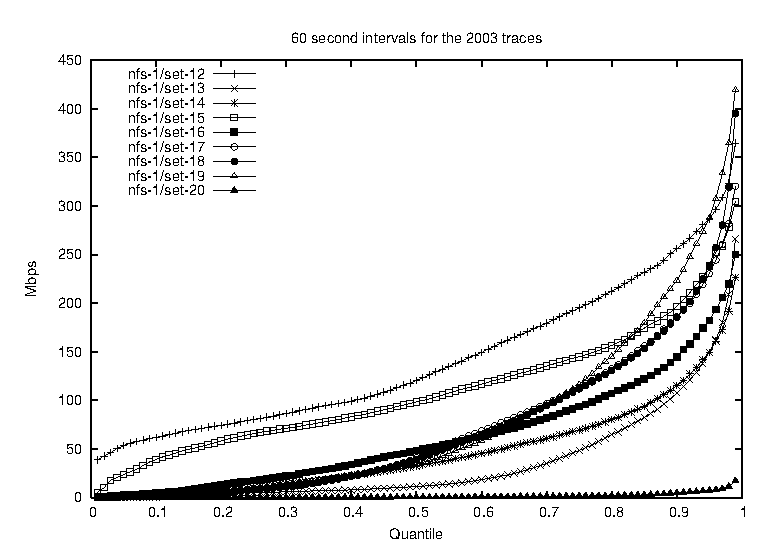
\epsfig{width=2.1in, angle=0, file=graphs/Mbps-nfs-1.ps}
%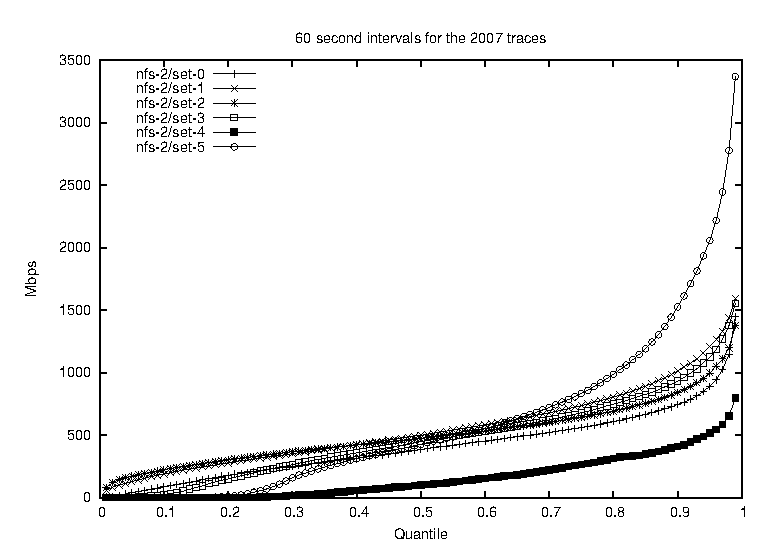
\epsfig{width=3.2in, angle=0, file=graphs/Mbps-nfs-2.ps}
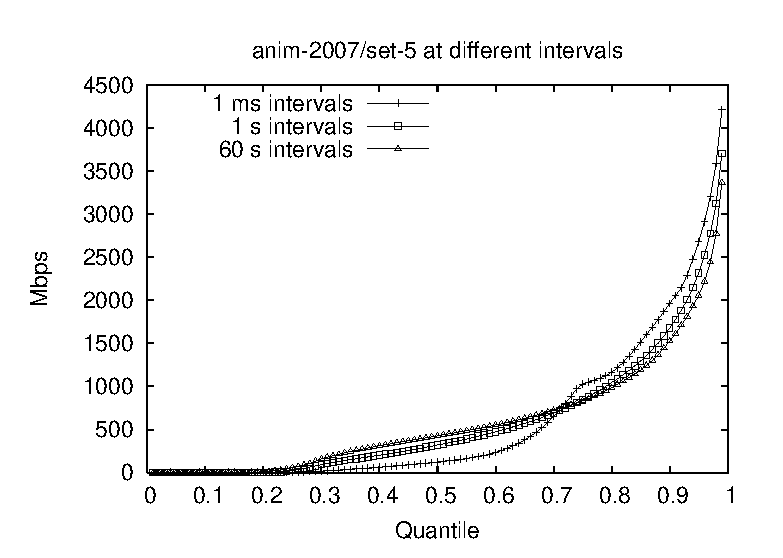
\epsfig{width=3.3in, angle=0, file=graphs/Mbps-nfs-2-set-5.ps}
\epsfig{width=3.3in, angle=0, file=graphs/Mbps-tails.ps}
\caption{Bandwidth measured in the collection process.  In figure (b),
animation-2007/set-5 at different intervals is the top group of 4 lines, and
animation-2003/set-12 is the bottom group of 4 lines. With 60s intervals, 
animation-2003/set-12 does not show the 0.9999 quantile 
because there were insufficient data points.}
\label{fig:bwrolling-mbps}
\end{figure*}

% \begin{figure*}
% 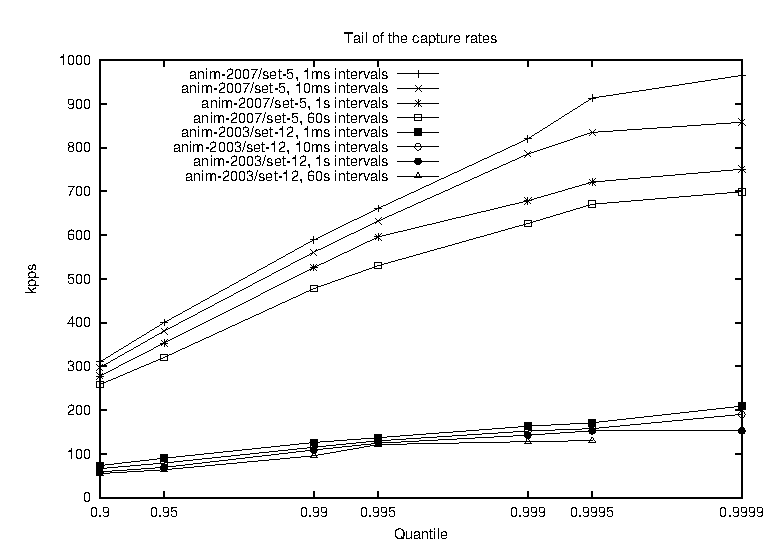
\epsfig{width=2.1in, angle=0, file=graphs/kpps-tails.ps}
% \caption{Tail of the quantiles in Mbps and kpps for the animation-2007 traces.}
% \label{fig:capture-tails}
% \end{figure*}

\subsection{Basic NFS analysis}

% nfs_hostinfo_rates, nfs_hostinfo_rate_quantiles, nfs_hostinfo_cube;
% choose sets nfs-2/set-[2,5]; nfs-1/set-[5,12]
%                     03+10, 06+13 ; 20+42, 27+49

% select from_unixtime(group_time), group_count/3600 where dataset = 'nfs-1/set-12' and group_time is not null and host is null  and operation is null and direction is null and op_dir is null
% nfs-1/set-5: 2003-09-16 .. 2003-09-18
% nfs-1/set-12: 2003-12-09 - 2003-12-10
% nfs-2/set-2: 2007-03-05 .. 2007-03-11
% nfs-2/set-5: 2007-10-12 .. 2007-10-17
% from hostinfo.hg + a few minor tweaks (n/a) for set-5 readdirplus
\begin{table*}
\begin{tabular}{|r||r|r||r|r||r|r||r|r|}
\hline
  & \multicolumn{2}{c||}{animation-2003/set-12} & \multicolumn{2}{c||}{animation-2003/set-5} & \multicolumn{2}{c||}{animation-2007/set-2} & \multicolumn{2}{c|}{animation-2007/set-5} \\
   operation &   Mops & bytes/op &   Mops & bytes/op &   Mops & bytes/op &   Mops & bytes/op \\
\hline
%     symlink &     0.008 &   201 &     0.000 &    92 &     0.001 &   415 &     0.000 &   458 \\
%       rmdir &     0.204 &   152 &     0.001 &    64 &     0.020 &   167 &     0.002 &   178 \\
%       mkdir &     0.173 &   304 &     0.005 &   193 &     0.071 &   336 &     0.004 &   334 \\
%      rename &     0.028 &   270 &     0.002 &   150 &     0.250 &   367 &     0.055 &   348 \\
%\hline
%      fsinfo &     0.023 &   176 &     0.003 &    72 &     1.352 &   176 &     0.619 &   176 \\
%        link &     0.000 &    86 &     0.000 &    88 &     3.259 &   314 &     0.182 &   322 \\
%        null &     0.259 &     5 &     0.087 &     4 &     1.482 &     4 &     2.808 &     4 \\
%      create &     0.296 &   295 &     0.965 &   200 &     4.639 &   367 &     1.616 &   344 \\
%\hline
%      remove &     0.275 &   136 &     0.641 &    69 &     8.419 &   194 &     1.500 &   186 \\
%     setattr &     0.716 &   133 &     1.075 &   136 &     9.415 &   193 &     6.531 &   192 \\
     readdir &     4.579 &   281 &     1.132 &  3940 &    28.318 &  4089 &    18.350 &  4071 \\
 readdirplus &     0.632 &  2307 &     0.000 &  n/a  &    32.806 &  1890 &    20.271 &  2001 \\
    readlink &     0.081 &    74 &     0.049 &    79 &    25.421 &   204 &    42.335 &   203 \\
      fsstat &    19.875 &    56 &    50.416 &    56 &     0.017 &   180 &     0.003 &   180 \\
       write &    14.546 &  9637 &    30.236 &  7880 &    32.390 & 13562 &    45.177 & 15015 \\
\hline
      lookup &   134.108 &    83 &    82.823 &    92 &   643.854 &   239 &   807.127 &   235 \\
        read &   345.743 &  1231 &   165.969 &  7855 &  1460.669 & 14658 &  1761.199 & 12301 \\
      access &     1.858 &   136 &     0.000 &   136 &  4000.204 &   136 &  3570.404 &   136 \\
     getattr &   244.650 &   104 &   967.961 &   104 &  6598.515 &   124 &  2756.785 &   123 \\
\hline
 {\bf total} &   768.053 &   790 &  1301.364 &  1274 & 12851.102 &  1833 &  9034.968 &  2599 \\
\hline
\end{tabular}

\caption{symlink, rmdir, mkdir, and rename were pruned as there were
fewer than 1 million operations; fsinfo, link, null, create, remove,
and setattr were pruned as there were fewer than 10 million
operations.  The Mops column could be calculated from nfsstat, but the
bytes/op column could not.}

\label{table:nfs-stats-overview}
\end{table*}

\begin{figure*}
% 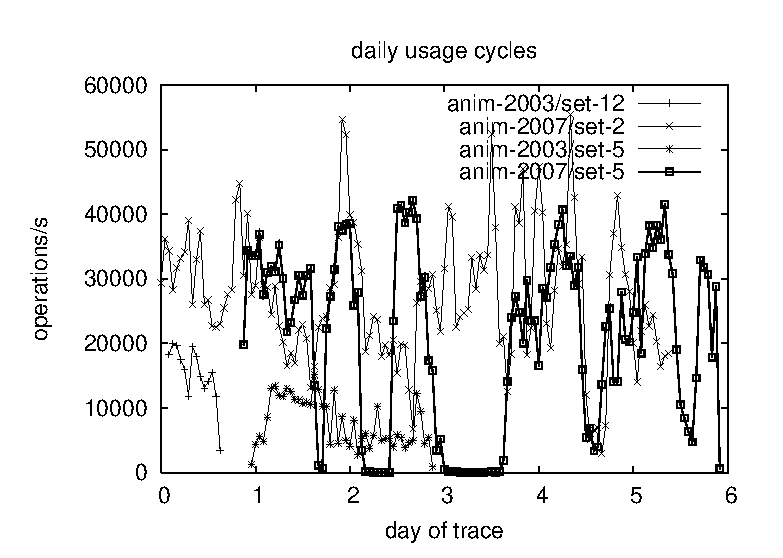
\epsfig{width=2.1in, angle=0, file=graphs/daily-oprate.ps}
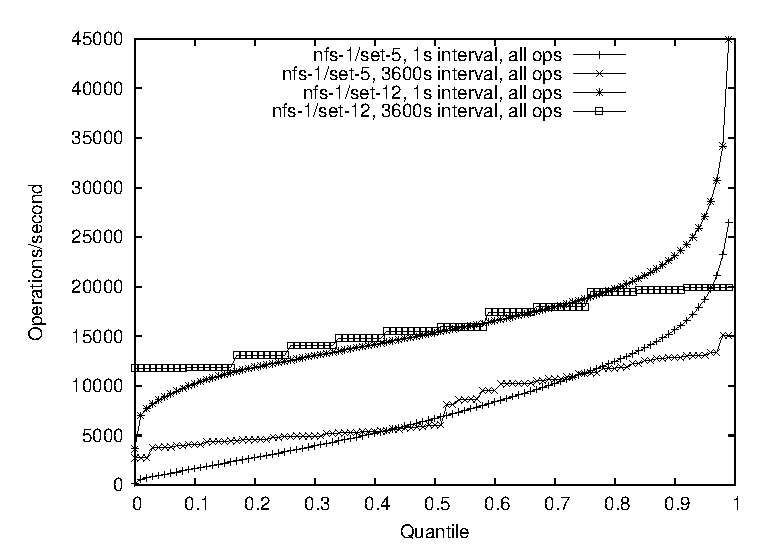
\epsfig{width=3.3in, angle=0, file=graphs/allops-quantile-nfs-1.ps}
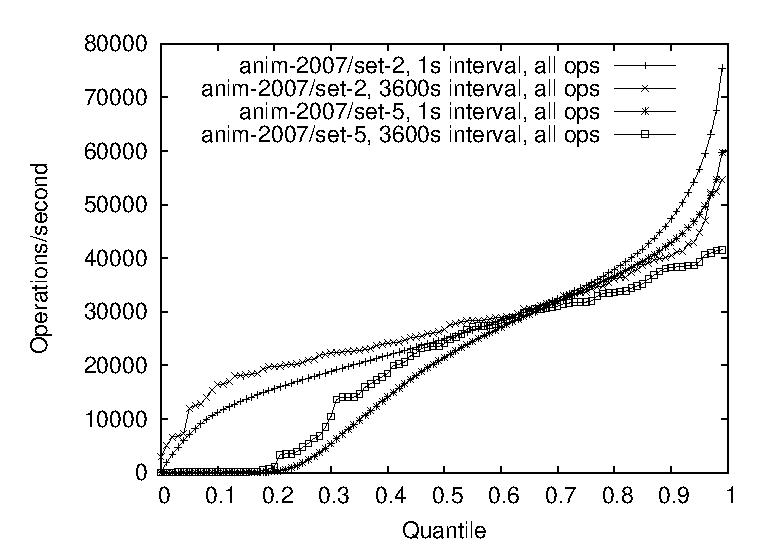
\epsfig{width=3.3in, angle=0, file=graphs/allops-quantile-nfs-2.ps}
\caption{Operation rates, as quantiles for anim-2003, anim-2007.}
\label{fig:oprates}
\end{figure*}

\begin{figure*}
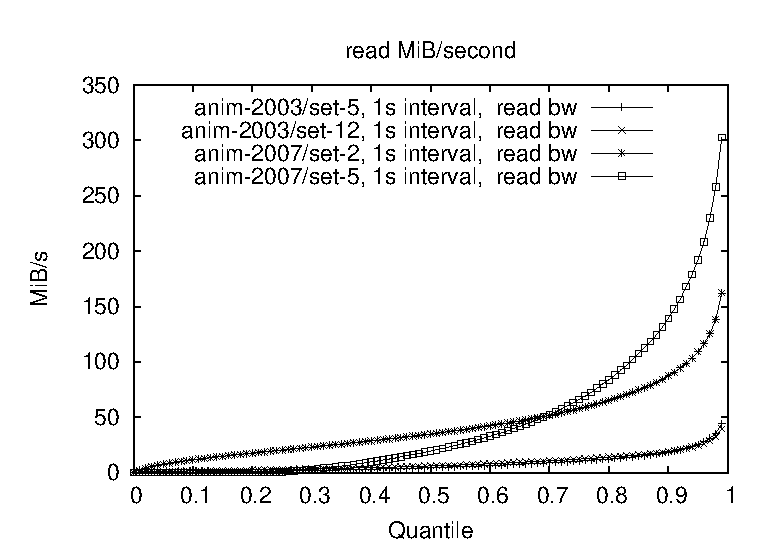
\epsfig{width=3.3in, angle=0, file=graphs/bw-read.ps}
%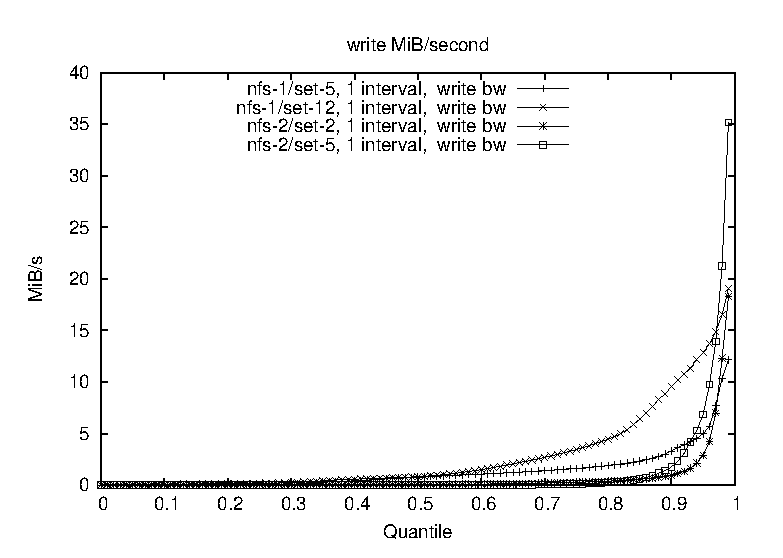
\epsfig{width=2.1in, angle=0, file=graphs/bw-write.ps}
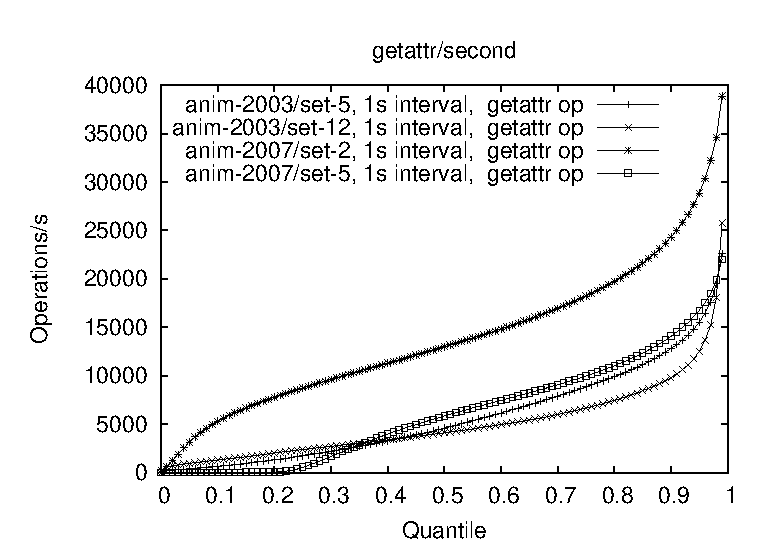
\epsfig{width=3.3in, angle=0, file=graphs/ops-getattr.ps}
\caption{Bandwidth for reads and operation rate for getattrs in the four traces.}
\label{fig:bw-ops-quantiles}
\end{figure*}

Examining the overall set of operations used by a workload provides
insight into what operations need to be optimized to support the
workload.  Examining the distribution of rates for the workload tells
us if the workload is bursty, and hence we need to handle a higher
rate than would be implied by mean arrival rates, and if there are
periods of idleness that could be exploited.

Table~\ref{table:nfs-stats-overview} provides an overview of all the
operations that occurred in the four traces we are examining in more
detail.  It shows a number of substantial changes in the workload
presented to the NFS subsystem.  First, the read and write sizes have
almost doubled from the animation-2003 to animation-2007 datasets.  This is expected
because the company moved from NFSv2 to NFSv3 between the two
tracing periods, and set the v3 read/write size to 16k.  We asked and
were told they set it to those sized based on some performance
measurements of sequential I/O.  The NFS version switch also accounts
for the increase in access calls (new in v3), and readdirplus (also
new in v3).  

We also see that this workload is incredibly read-heavy.  This is
expected; the animation workload reads a very large amount of
textures, models, etc. to produce a relatively small output frame.
However, we believe that our traces under-estimate the number of write
operations.  We discuss the write operation underestimation below.
The abnormally low read size for set-12 occurred because
that server was handling a large number of stale FH requests.  The
replies were therefore small and pulled down the bytes/operation.  We
see a lot more getattr operations in set-5 than set-12 because set-12
is a server behind some nfs-caches, whereas set-5 is the workload
before the nfs-caches.

Table~\ref{table:99quant-differences} and
figure~\ref{fig:oprates}(a,b) show how long averaging intervals can
distort the load placed on the storage system.  If we were to develop
a storage system for the hourly loads reported in most papers, we
would fail to support the substantially higher near peak (99\%) loads
seen in the data.  It also hides periods of idleness that could be
used for incremental scrubbing and data reorganization.  We do not
include the traditional graph of ops/s vs time because our workload
does not show a strong daily cycle.  Animation companies tend to run
batch processing overnight, and interactive jobs during the day, so
show much more constant load on the cluster.  The only observable
pattern is that weekends usually drop off to zero.

Figure~\ref{fig:bw-ops-quantiles} shows the read operation MiB/s and
the getattr operations/s.  It shows that relative to the amount of
data being transferred, the number of getattrs has been reduced,
likely a result of the transition from NFSv2 to NFSv3.  The graph
shows the payload data transferred, so it includes the offset and
filehandle of the read request, and the size and data in the reply,
but does not include IP headers or NFS RPC headers.  It shows that the
NFS system is driven heavily, but not excessively. The write graph
(not shown for space reasons) implies that the write bandwidth has
gotten more bursty, but has stayed roughly constant.

This result led us to further analyze the data.  We were surprised
that that write bandwidth would not increase, even though it is not
implausible as the frame output size has not increased.  We analyzed
the traces to look for missing operations in the sequence of
transaction ids, automatically inferring if the client is using a
big-endian or little-endian counter.  The initial results looked quite
good, animation-2007/set-2 showed 99.7\% of the operations were in sequence,
animation-2007/set-5 showed 98.4\%, and counting the skips of 128 transactions
or less, we found only 0.21\% and 0.50\% respectively (the remaining
entries were duplicates or ones that we could not positively tell if
they were in sequence or a skip).  However, when we looked one level
deeper at the operation that preceded a skip in the sequence, we found
that 95\% of the skips followed a write operation for set-2, and 45\%
for set-5.  The skips in set-2 could increase the write workload by a
factor of 1.5x if all missing skips after writes are associated with
writes.  We expected a fair number of skips for set-5 since we
experienced packet loss under load, but we did not expect it for
set-2. \fix{run analysis on full dataset, determine how much we were hurt.  
On one file it was <10\%}

Further examination indicated that the problem came about because we
followed the same parsing technique for TCP packets as was used in
nfsdump2~\cite{ellardTraces}.  We started at the beginning of the
packet and parsed all of the RPCs that we found that matched all
required bits to be RPCs.  Unfortunately, over TCP, two back to back
writes will not align the second write RPC with the packet header, and
we will miss subsequent operations until they re-align with the packet
start.  While the fraction of missing operations is small, they are
biased toward writes (read replies can only be affected if the second
read reply is close enough to the first that they are combined).  This
leads us to one of our lessons, extensive validation of the conversion
tool is important.  Both validation through validation statistics, and
through the use of a known workload that exercises the capture tools.
\fix{Clarify that we mean replay a trace and verify what is captured
from replay is what was replayed -- verify the capture side, not the
replay side} An NFS replay tool~\cite{NingningFast05} could be used to
validate that the captured workload is the one that was replayed.
This comparison has been done to validate a block based replay
tool~\cite{AndersonFast04}, but has not been done to validate a
capture tool, as that work simply assumed capture was correct.
\fix{create analysis that compares timing of ops to packets and
estimates missing writes if we can get the space for it}
% We can therefore use
% the timing information from requests and replies to identify gaps in
% the dataset and determine how many bytes were skipped.  This will
% allow us to approximate the number of missing writes.  Preservation of
% lower level information is a lesson we got right, and it will allow us
% to partially reconstruct flaws in the traces.  
We believe a similar
flaw is present in earlier traces~\cite{ellardTraces} because the same
parsing technique was used, although we do not know how much those traces were
affected.

% select dataset, group_seconds, operations_per_second from xnfs_hostinfo_rate_quantiles where host is null and direction = 'send' and operation is null and op_dir is null and quantile = 0.99
\begin{table}
\begin{tabular}{|l|r|r|r|}
\hline
dataset & 1s ops/s & 3600s ops/s & ratio \\
\hline
anim-2003/set-5  & 26,445 & 15,110 & 1.75x \\
anim-2003/set-12 & 44,926 & 19,923 & 2.25x \\
anim-2007/set-2  & 75,457 & 54,657 & 1.38x \\
anim-2007/set-5  & 59,727 & 41,550 & 1.44x \\
\hline
\end{tabular}
\caption{Ratio between operation rates at 1 second and one hour grouping sizes}
\label{table:99quant-differences}
\end{table}

\subsection{File sizes}

\begin{figure}
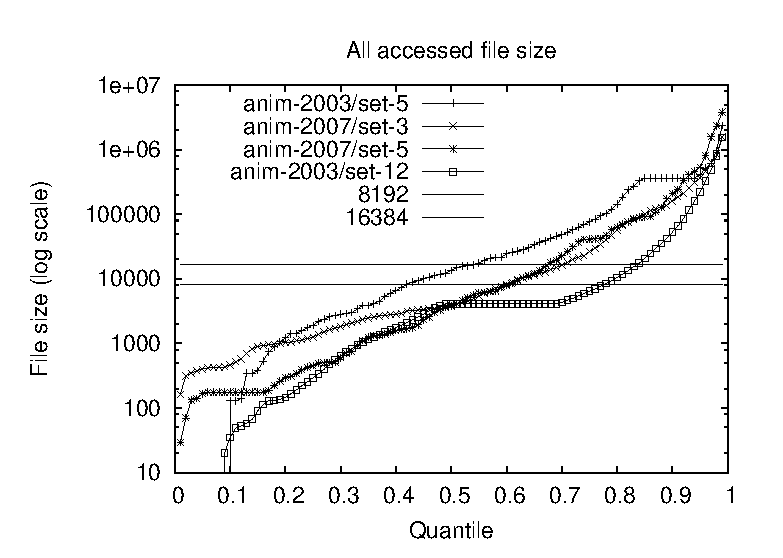
\epsfig{width=3.2in, angle=0, file=graphs/file-size.ps}
\caption{File size distribution for all accessed files.}
\label{fig:file-size}
\end{figure}

File sizes affect the potential internal fragmentation for a
filesystem.  They affect the maximum size of I/Os that could be
executed, and they affect the potential sequentiality in a workload.

Figure~\ref{fig:file-size} shows the size of files accessed in our
traces.  It shows that the files in the animation workload are in
general very small, as 40-80\% of the files are smaller than 8k, and
hence will be read in a single I/O for the 2003 traces.  70\% of the
files are smaller than 16k for the 2007 traces, and hence will be read
in a single I/O.  While there are larger files in the traces, 99\% of
the files are smaller than 10MB.  The small file sizes present in this
workload, and the preponderance of writes suggest that a flash file
system~\cite{Kawaguchi95aflash-memory} or MEMS file
system~\cite{SchlosserFast04} could support a substantial portion of
the workload.

\subsection{Sequentiality}

\begin{figure*}
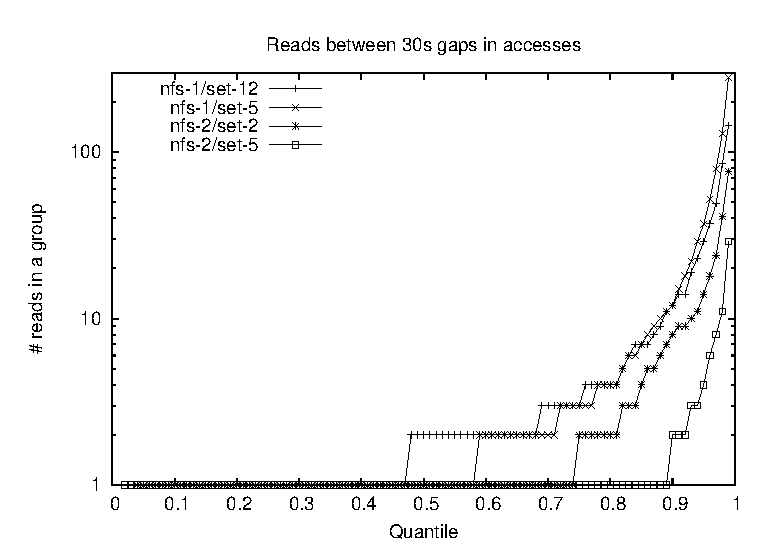
\epsfig{width=3.3in, angle=0, file=graphs/seq-read-group-counts.ps}
% 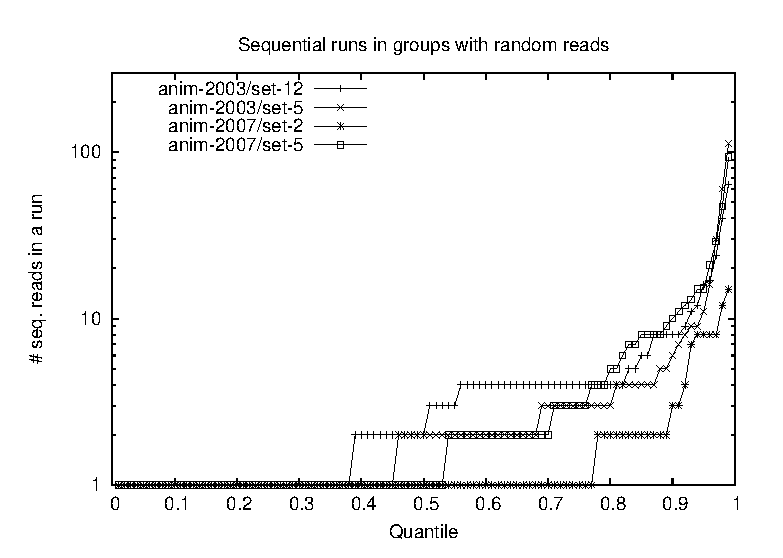
\epsfig{width=2.1in, angle=0, file=graphs/seq-in-random-seq-count.ps}
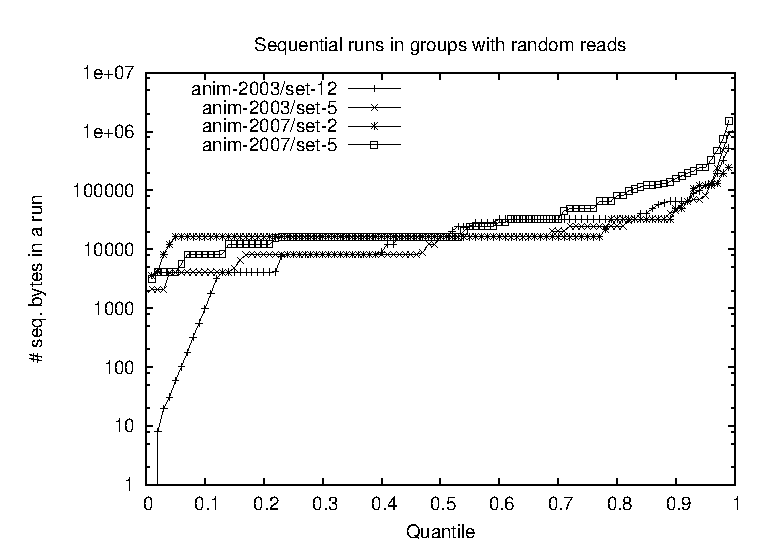
\epsfig{width=3.3in, angle=0, file=graphs/seq-in-random-seq-bytes.ps}
\caption{number of reads in a single group (more than 30s gap between I/Os); }
\label{fig:seq-analysis}
\end{figure*}

\begin{figure}
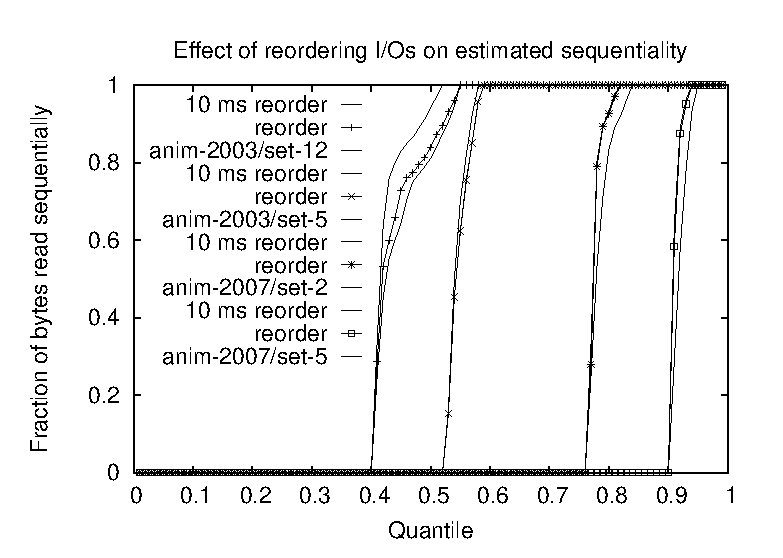
\epsfig{width=3.2in, angle=0, file=graphs/seq-bytes-compare.ps}
\caption{Each group of lines shows how the estimated sequentiality was
affected by allowing either reordering of I/Os within 10ms of the
reply, reordering within the request-reply window, or no reordering.
The small horizontal difference between the lines shows that reordering for
this workload has a negligable effect on sequentiality.}
\label{fig:seq-bytes-compare}
\end{figure}

Sequentiality is one of the most important properties for storage
systems because disks are much more efficient when handling sequential
data accesses.  Prior work has presented
various methods for calculating sequentiality.  Both
Ellard~\cite{EllardFast03} and Leung~\cite{LeungUsenix08} split accesses
into groups and calculate the sequentiality within the group.  Ellard
emulates opens and closes by looking for 30s groups in the access
pattern.  Ellard tolerates small gaps in the request stream as
sequential, e.g. an I/O of 7k at offset 0 followed by an I/O of 8k at
offset 8k would be considered sequential.  Ellard also re-orders I/Os
to deal with client-side reordering. In particular Ellard looks
forward a constant amount from the request time to find I/Os that
could make the access pattern more sequential.  This constant was
determined empirically.  Leung treats the first I/O after an open as
sequential.

We prefer to only reorder within overlapping requests. Given two I/Os,
A, and B, if the request-reply intervals overlap, then we are willing
to re-order the requests to improve estimated sequentiality.  We
believe this is a better model because the NFS server could 
re-order those I/Os.  In practice
figure~\ref{fig:seq-bytes-compare} shows that for our traces this
reordering makes little difference.  Allowing reordering an additional
10ms beyond the reply of I/O A slightly increases the sequentiality,
but generally not much more than just for overlapping requests.

We also decide on whether the first I/O is sequential or random based
on additional I/Os.  If the second I/O (after any reordering) is
sequential to the first one, than the first I/O is sequential,
otherwise it is random.  If there is only one I/O to a particular
file, then we consider the I/O to be random since the NFS server would
have to reposition to that file to start the read.  

Given our small file sizes, it turns out that most accesses count as
random because they read the entire file in a single I/O.  We can see
this in figure~\ref{fig:seq-analysis}(a) which shows the number of
reads in a group.  Most groups are single I/O groups (70-90\% in the
2007 traces).  We see about twice as many I/Os in the 2003 traces,
because the I/Os in the 2003 traces are only 8KiB rather than 16KiB.

Sequential runs within a random group turns out to be more
interesting.  Figure~\ref{fig:seq-analysis}(b) show the number of
bytes accessed in sequential runs within a
random group.  We can see that if we start accessing a file at random,
most (50-80\%) of the time we will do single or double I/O accesses (8-32k).
However we can also see that we can get some extended runs within a
random group, although 99\% of the runs are less than 1MB.

% select dataset,operation, max(mean_operations_per_second) from xnfs_hostinfo_rates where group_seconds = 1 and host is null and direction = 'send' and operation is not null and op_dir is null and mean_operations_per_second > 300 group by dataset,operation order by operation
% --> access, fsstat, getattr, lookup, read, write 


\section{Conclusions}
\label{sec:conclusion}

We have described three improved techniques for packet capture on
networks.  The easily adopted technique should allow anyone capturing
NFS, CIFS, or iSCSI traffic from moderate performance storage systems
($<=$1Gbit) to capture traffic with no losses.  The most advanced
technique allows lossless capture for 5-10Gbit storage systems, which
is at the high end of most file storage systems. 

We have provided guidelines for conversion, namely in terms of
parallelizing the conversion, retaining low level information, using
reversable anonymization when possible, and most importantly tagging
the trace data with version information to handle conversion bugs.

We have described our binary storage format that uses chunked
compression with multiple possible compression techniques, the use of
typed relational-style data structuring, the use of delta encoding,
and the use of type-safe, high-speed accessors.

We have explained the cube, and approximate quantile techniques that
we adopted from the database literature to handle analysis of very
large data sets.  We have also explained our hashtable, rotating
hash-map, and plotting techniques that we use for analyzing the data.

We have analyzed our NFS workload examining some of the different
properties found in a feature animation workload and demonstrating
that our techniques are effective.  Finally, we have made our traces
and tools available at http://anonymized.example.com


\bibliography{references}
\bibliographystyle{plain}

% http://ieeexplore.ieee.org/Xplore/login.jsp?url=/iel5/9595/30315/01392983.pdf?temp=x

\end{document}







